\documentclass[handout]{beamer}
%Пакеты для математических символов:
\usepackage{amsmath} % американское математическое сообщество.
\usepackage{amssymb} % миллион разных значков и готический, ажурный шрифты.
\usepackage{amscd} % диаграммы, графики.
\usepackage{amsthm} % окружения теорем, определений и тд.
\usepackage{physics} % основные физические символы
%\usepackage{latexsym} % треугольники и пьяная стрелка.

%пакеты для шрифтов:
%\usepackage{euscript} % прописной шрифт с завитушками.
\usepackage{MnSymbol} % Значеки доказательства
\usepackage{verbatim} % улучшенный шрифт "пишущей машинки".
%\usepackage{array} % более удобные таблицы.
%\usepackage{multirow} % мультистолбцы в таблицах.
%\usepackage{longtable} % таблицы на несколько страниц.
%\usepackage{latexsym}

\usepackage{etoolbox}
\usepackage{slashbox} %Разделениени текста \backslashbox{}{}
\usepackage{collectbox} % Добавляет коробочки, можно складывать туда текст)

%Пакеты для оформления:
\RequirePackage[center, medium]{titlesec}% Стиль секций и заголовков
%\usepackage[x11names]{xcolor} % 317 новых цветов для текста.
%\usepackage{multicol} % набор текста в несколько колонн.
\usepackage{graphicx} % расширенные возможности вставки стандартных картинок.
\usepackage{subcaption} % возможность вставлять картинки в строчку
%\usepackage{caption} % возможность подавить нумерацию у caption.
\usepackage{wrapfig} % вставка картинок и таблиц, обтекаемых текстом.
\usepackage{cancel} % значки для сокращения дробей, упрощения, стремления.
%\usepackage{misccorr} % в заголовках появляется точка, но при ссылке на них ее нет.
%\usepackage{indentfirst} % отступ у первой строки раздела
%\usepackage{showkeys} % показывает label формул над их номером.
%\usepackage{fancyhdr} % удобное создание верхних и нижних колонтитулов.
%\usepackage{titlesec} % еще одно создание верхних и нижних колонтитулов

%Пакеты шрифтов, кодировок. НЕ МЕНЯТЬ РАСПОЛОЖЕНИЕ.
\usepackage[utf8]{inputenc} % кодировка символов.
%\usepackage{mathtext} % позволяет использовать русские буквы в формулах. НЕСОВМЕСТИМО С tempora.
\usepackage[T1, T2A]{fontenc} % кодировка шрифта.
\usepackage[english, russian]{babel} % доступные языки.



%Отступы и поля:
%размеры страницы А4 11.7x8.3in
\textwidth=7.3in % ширина текста
\textheight=10in % высота текста
\oddsidemargin=-0.5in % левый отступ(базовый 1дюйм + значение)
\topmargin=-0.5in % отступ сверху до колонтитула(базовый 1дюйм + значение)


%Сокращения
%Скобочки
\newcommand{\inrad}[1]{\left( #1 \right)}
\newcommand{\inner}[1]{\left( #1 \right)}
\newcommand{\infig}[1]{\left{ #1 \right}}
\newcommand{\insqr}[1]{\left[ #1 \right]}
\newcommand{\ave}[1]{\left\langle #1 \right\rangle}


%% Красивые <= и >=
\renewcommand{\geq}{\geqslant}
\renewcommand{\leq}{\leqslant}

%%Значек выполнятся
\newcommand{\per}{\hookrightarrow}


%% Более привычные греческие буквы
\renewcommand{\phi}{\varphi}
\renewcommand{\epsilon}{\varepsilon}
\newcommand{\eps}{\varepsilon}
\newcommand{\com}{\mathbb{C}}
\newcommand{\re}{\mathbb{R}}
\newcommand{\nat}{\mathbb{N}}
\newcommand{\stp}{$\filledmedtriangleleft$}
\newcommand{\enp}{$\filledmedsquare$}

\makeatletter
\newcommand{\sqbox}{%
    \collectbox{%
        \@tempdima=\dimexpr\width-\totalheight\relax
        \ifdim\@tempdima<\z@
            \fbox{\hbox{\hspace{-.5\@tempdima}\BOXCONTENT\hspace{-.5\@tempdima}}}%
        \else
            \ht\collectedbox=\dimexpr\ht\collectedbox+.5\@tempdima\relax
            \dp\collectedbox=\dimexpr\dp\collectedbox+.5\@tempdima\relax
            \fbox{\BOXCONTENT}%
        \fi
    }%
}
\makeatother
\newcommand{\mergelines}[2]{
\begin{tabular}{llp{.5\textwidth}}
#1 \\ #2
\end{tabular}
}
\newcommand\tab[1][0.51cm]{\hspace*{#1}}
\newcommand\difh[2]{\frac{\partial #1}{\partial #2}}


\usetheme{Madrid} % Выбор темы
\usecolortheme{default} % Выбор цветовой схемы
\title{Волновая пластинка $\lambda/2$}
\author{Карибджанов Матвей}

\begin{document}



\begin{frame}% первый слайд
    \titlepage
\end{frame}

\begin{frame}
    \frametitle{Основные свойство}
    \begin{columns}
        \begin{column}{0.5\textwidth}
            \begin{equation*}
                D = \epsilon E \ \to \ D = \hat \epsilon E
            \end{equation*}

            \begin{gather*}
                \hat \epsilon = 
                \begin{pmatrix}
                    \epsilon_f & 0 & 0 \\
                    0 & \epsilon_f & 0 \\
                    0 & 0 & \epsilon_s
                \end{pmatrix}
            \end{gather*}
            
            \begin{equation*}
                \insqr{k, \insqr{k, E}} = 
                \cfrac{\omega}{c} \insqr{k, H}
            \end{equation*}
            \begin{equation*}
                k \inner{k, E} - k^2 E 
                = - \cfrac{\omega^2}{c^2} \vb D
            \end{equation*}

            \begin{equation*}
                \cfrac{1}{n^2} = \cfrac{\inner{E, D}}{D^2} = \cfrac{D\epsilon^{-1}D}{D^2}    
            \end{equation*}
            
        \end{column}
        \begin{column}{0.5\textwidth}
            \begin{figure}[h]
                \centering
                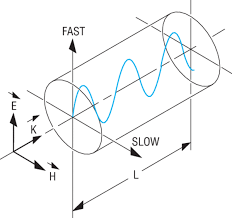
\includegraphics[width=0.6\textwidth]{wp.png}
            \end{figure}
            
            \begin{gather*}
                \begin{pmatrix}
                    E_1 cos(\omega t) \\
                    E_2 cos(\omega t)
                \end{pmatrix}
                \implies
                \begin{pmatrix}
                    E_1 cos(\omega t) \\
                    E_2 cos(\omega t + k\delta)
                \end{pmatrix}
            \end{gather*}
            
            \begin{equation*}
                \delta = L (n_f^2 - n_s^2), \quad \delta = \pi \implies \frac{\lambda}{2}
            \end{equation*}
        \end{column}
      \end{columns}
\end{frame}


\begin{frame}
    \frametitle{Требования}
    \begin{columns}
        \begin{column}{0.5\textwidth}
            Кртерии от основного свойства 
            \begin{itemize}
                \item Диапазон $n(a)$
                \item Нормальные условия
            \end{itemize}
        \end{column}
        
        \begin{column}{0.5\textwidth}
            Общии критерии 
            \begin{itemize}
                \item Коэффициент отражения
                \item Качество поверхности
                \item Размеры
                \item Геометрия
            \end{itemize}
        \end{column}
    \end{columns}

    \begin{figure}[h]
        \centering
        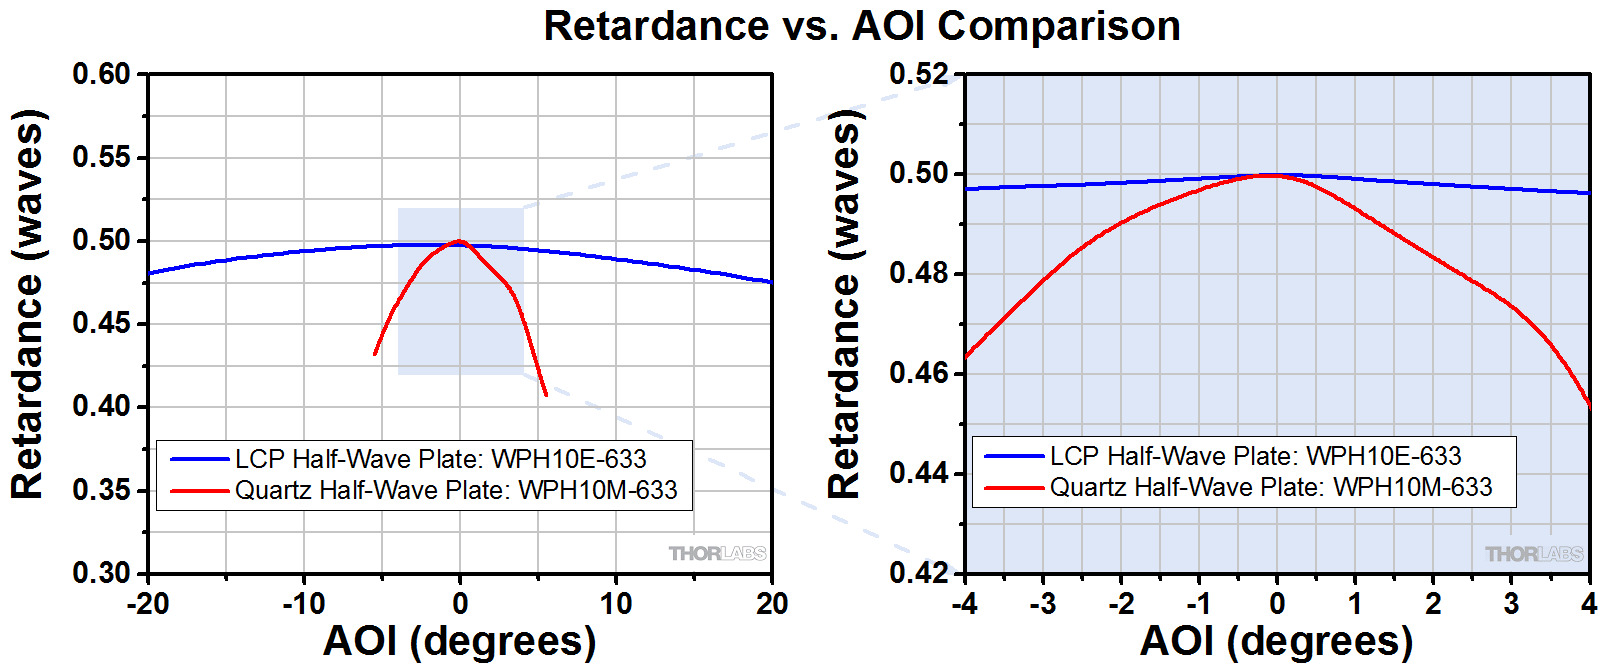
\includegraphics[width=0.8\textwidth]{n_w.jpg}
    \end{figure}

\end{frame}

\begin{frame}
    \frametitle{12.7mm Dia. 355nm $\lambda / 2$ Quartz Waveplate Multiple Order}
    \begin{columns}
        \begin{column}{0.5\textwidth}
            \begin{tabular}{c||c}
                Качество поверхности & 10-5 S-D \\ \hline
                $\lambda$ & 355 nm \\ \hline
                Откленение & $\pm \lambda /200$ \\ \hline
                Угол & 0.5 arcsec \\ \hline
                D & 12.70 mm \\ \hline
                Темп. коэф. &  $ 0.0015  \lambda / ^\circ C$
            \end{tabular}
        \end{column}

        \begin{column}{0.5\textwidth}
            \begin{figure}[h]
                \centering
                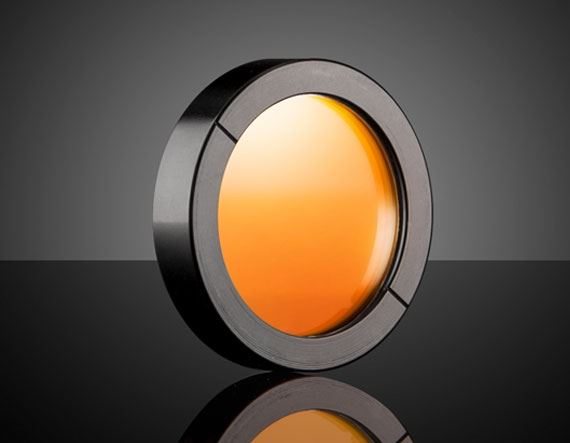
\includegraphics[width=0.8\textwidth]{1.jpg}
            \end{figure}
        \end{column}
    \end{columns}

    Цена: \href{https://www.edmundoptics.com/p/127mm-dia-355nm-lambda2-quartz-waveplate-multiple-order/28055/}{252 \$}
\end{frame}

\begin{frame}
    \frametitle{ 76.2mm Dia. 532nm $\lambda /2$ Quartz Waveplate Zero Order }
    \begin{columns}
        \begin{column}{0.5\textwidth}
            \begin{tabular}{c||c}
                Качество поверхности & 10-5 S-D \\ \hline
                $\lambda$ & 532 nm \\ \hline
                Откленение & $\pm \lambda /200$ \\ \hline
                Угол & 0.5 arcsec \\ \hline
                D & 76.20  mm \\ \hline
                Темп. коэф. &  $0.0001 \lambda / ^\circ C$
            \end{tabular}
        \end{column}
    \end{columns}

    Цена: \href{https://www.edmundoptics.com/p/762mm-dia-532nm-lambda2-quartz-waveplate-zero-order/28042/}{2,265 \$}
\end{frame}

\begin{frame}
    \frametitle{  12.7mm Dia. 488nm $\lambda /2$ Quartz Waveplate Multiple Order }
    \begin{columns}
        \begin{column}{0.5\textwidth}
            \begin{tabular}{c||c}
                Качество поверхности & ? S-D \\ \hline
                $\lambda$ & 532 nm \\ \hline
                Откленение & $\pm \lambda /250$ \\ \hline
                Угол & 3 arcsec \\ \hline
                D & 25.00  mm \\ \hline
                Темп. коэф. &  $ ? \lambda / ^\circ C$
            \end{tabular}
        \end{column}
    \end{columns}

    Цена: \href{https://www.edmundoptics.com/p/532nm-lambda2-polymer-waveplate/32495/}{431 \$}
\end{frame}

\end{document}